\documentclass[preprint,12pt]{article}
\usepackage{url}
\usepackage{cite}
\usepackage{epsfig}


\begin{document}

\begin{figure}[h]
\centering
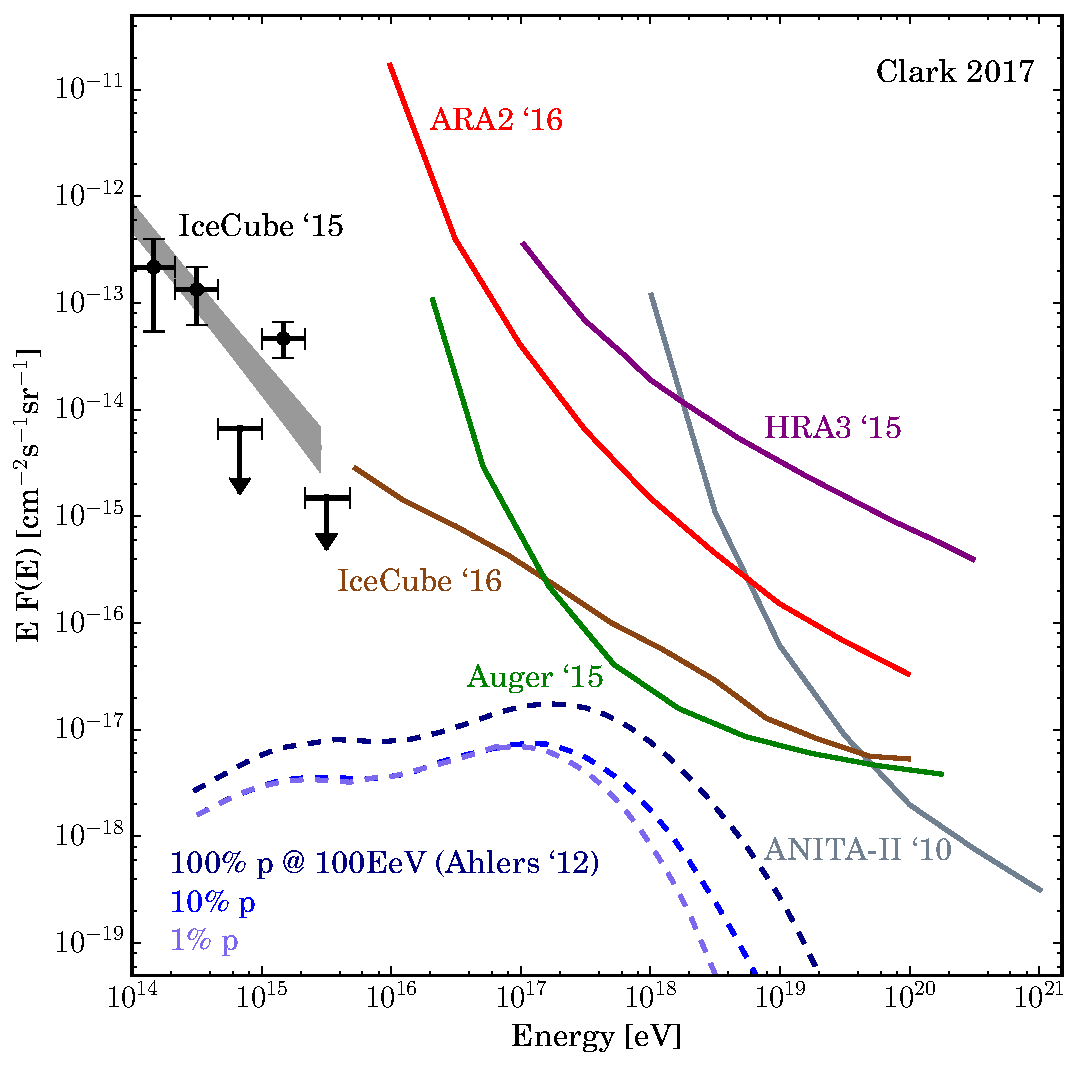
\includegraphics[width=.9\textwidth]{leading_limits_plot.pdf}
\caption{A plot of the latest published limits and flux measurements from various ultra-high energy neutrino experiments. The data and spectral fit are from IceCube \cite{IceCube2015, IceCube2016}, Pierre Auger \cite{Auger2015}, ARA \cite{Ara2016}, ARIANNA \cite{Arriana2015}, and ANITA-II \cite{Anita2010Erratum}. The models (dashed line) are from Ahlers \textit{et. al} \cite{Ahlers2012}. The Auger limit is a single-flavor only measurement.}
\label{fig:sigcondblock1}
\end{figure}

\newpage

The limit plot contains the following data sets:

\begin{itemize}
\item 2015 The Pierre Auger Limit. \url{https://arxiv.org/abs/1504.05397v2} \cite{Auger2015}.
\item 2016 IceCube Limit. \url{https://arxiv.org/abs/1607.05886} \cite{IceCube2016}.
\item 2015 IceCube Spectrum Data. \url{https://arxiv.org/abs/1507.03991}  \cite{IceCube2015}.
\item 2010 ANITA-II Limit. \url{https://arxiv.org/abs/1003.2961} \cite{Anita2010, Anita2010Erratum}.
\item 2016 ARA2 Limit. \url{https://arxiv.org/abs/1507.08991} \cite{Ara2016}.
\item 2015 ARIANNA HRA3 Limit. \url{https://arxiv.org/abs/1410.7352}. \cite{Arriana2015}.
\item 2012 Ahlers and Halzen models. \url{https://arxiv.org/abs/1208.4181}. \cite{Ahlers2012}.
\end{itemize}

\bibliographystyle{unsrt}
\bibliography{references} 

\end{document}
